	\chapter{Requirements}
	\label{cha:Requirements}
		% Allgemeine REQs an FW, RT (und evtl design-for-testability)
		% \section{Firmware-Requirements}
		All stakeholders of the OCTane decided in two meetings the requirements towards the OCTane and especially the firmware running on it. The fact, that the stakeholders, or, in other words, the users of the OCTane agreed on these, leads to the label 'user requirements'. Accompanying tags in the form 'RU-xx' allow for tracing relations between a requirement and according test-cases or points of implementation inside the source-code. %, as well as a traceability matrix
		\section{User requirements}
				
	% perl -p -e 's/RU-/"RU-".++$i/ge' _REQS.tex > REQS.tex

	\req{ RU-1 }{Basic Functionality}{}{}
	{ The FirmWare has to access available hardware, to generate two-channel signals in ramp-, constant or arbitrary form, with 
	\begin{itemize} \setlength\itemsep{1px}
	\item sample-rates ( $\ne$ signal-frequency) up to 250kSPS
	\item a resolution of 16bit
	\item resulting in $\pm$10 volts of output voltage
	\end{itemize}
	
	}
	{}{}{}{General}
	\begin{center}
	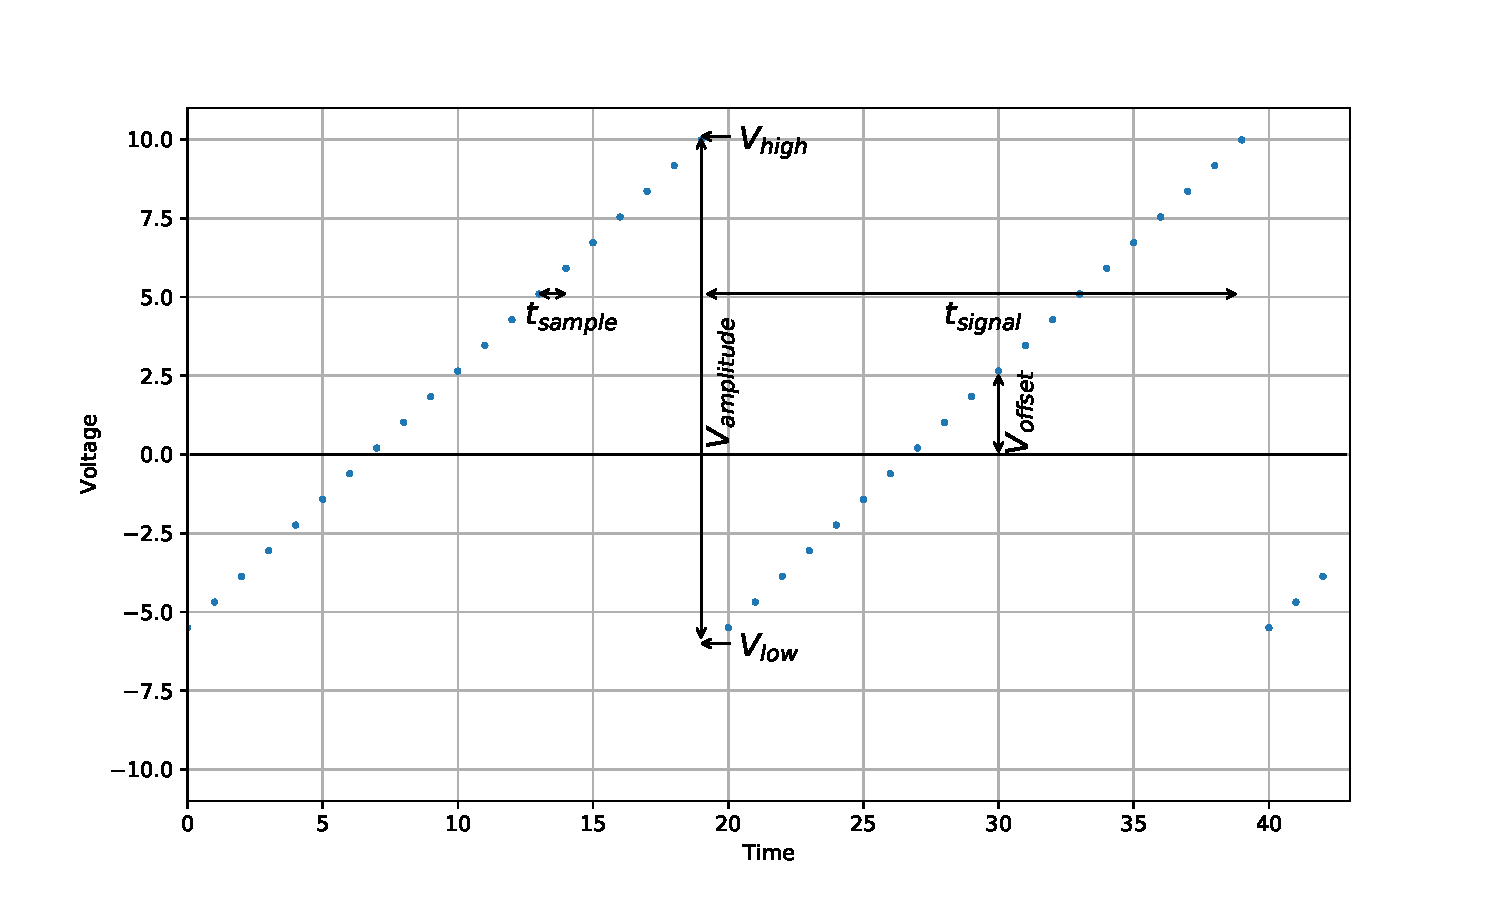
\includegraphics[width=0.99\textwidth, trim = {0 1.6cm 0 1.5cm}, clip]{src/_rampProperties.pdf}
	\end{center}
	\begin{align*}
	t_{sample} &\textrm{ ... sampling-time or -period, alias: trigger-rate } \\
	t_{signal} &\textrm{ ... signal-time or -period } \\
	f_{sample} &\textrm{ ... sampling-frequency or -rate } \\
	f_{signal} &\textrm{ ... signal-frequency or -rate } \\
	N &\textrm{ ... sample-count, length of the signal-vector } \\
	f_{sample} & = \frac{1}{t_{sample}} = N \cdot f_{signal} \\
	f_{signal} & = \frac{1}{t_{signal}} = \frac{1}{N \cdot t_{sample}} \\
	% f_{sample} & = N \times f_{signal} \\
	% t_{signal} & = N \times t_{sample}	\\
	% \end{align*}
	% \begin{align*}
	V_{amplitude} &\textrm{  ... difference between maximum and minimum voltage of a signal. } \\
	V_{offset} &\textrm{  ... deviation of a signal from 0 volts. } \\
	V_{high} &\textrm{  ... maximum voltage of a signal } \\
	V_{low} &\textrm{  ... minimum voltage of a signal } \\
	V_{amplitude} &= V_{high} - V_{low} \\ % \quad \quad V_{high} = V_{offset} + \frac{V_{amplitude}}{2} \\
	V_{offset} &= \frac{V_{high} + V_{low}}{2} \\ % \quad \quad V_{low} = V_{offset} - \frac{V_{amplitude}}{2} \\
	\rightarrow V_{high} &= V_{offset} + \frac{V_{amplitude}}{2} \quad V_{low} = V_{offset} - \frac{V_{amplitude}}{2}
	\end{align*}
	
	
	\req{ RI-5 }{Priorities}{}{}
	{ In case of temporal overlapping tasks, first priority lays with analogue signal generation, second prio with USB-connectivity, third prio with Miscellaneous functions. }
	{}{}{}{General}

	
	\req{ RU-2  }{Last Command Counts}{}{}
	{ The last submitted and accepted value for each parameter is the valid one.}
	{}{}{}{General}

	\req{ RU-3  }{Parameters}{}{}
	{ The FirmWare has to implement user-adjustable parameters according to Tab. 1. }
	{}{}{}{General}
	
	{	\scriptsize
					\begin{table}[H]
			\centering
			\scriptsize
			\begin{tabular}{l|p{65mm}|l|l|l}
			% \hline
			\redrow Parameter 	& Values						& reset value 	& Dim.		& Type 	\\ \hline
			TriggerA State		& off|idle|arm|run				& idle			& 			& enum	\\ \hline
			TrigA Mode			& finite|infinite (freerun)		& finite		& 			& enum	\\ \hline
			TrigA Input			& USB|ext|TrigB|butt0 			& TrigB			& 			& enum	\\ \hline
			TrigA Signal-Rate	& 100m ... 125k					& 30.00e3		& Hz		& float	\\ \hline
			TrigA Signal-Period	& 8u ... 10						& 3.33e-5		& s			& float	\\ \hline
			TrigA Size			& 0	... 250000	 				& 1000			& samples	& int	\\ \hline
			TriggerB State		& off|idle|arm|run 				& idle			& 			& enum	\\ \hline
			TrigB Signal-Rate	& 100m ... 125k					& 30			& Hz		& float	\\ \hline
			TrigB Mode			& finite|infinite (freerun)		& finite		& 			& enum	\\ \hline
			TrigB Input			& USB|ext|TrigC|butt1 			& TrigC			& 			& enum	\\ \hline
			TrigB Signal-Period	& 8u ... 10						& 3.33e-2		& s			& float	\\ \hline
			TrigB Size			& 0	... 250000	 				& 1000			& samples	& int	\\ \hline
			TriggerC State		& off|idle|arm|run				& idle			& 			& enum	\\ \hline
			TrigC Mode			& finite|infinite (freerun)		& finite		& 			& enum	\\ \hline
			TrigC Input			& USB|ext|butt2					& USB			& 			& enum	\\ \hline
			TrigC Signal-Rate	& 20m ... 125k					& 3e-2			& Hz		& float	\\ \hline
			TrigC Signal-Period	& 8u ... 50						& 33.33			& s			& float	\\ \hline
			TrigC Size			& 0 ... 250000					& 1				& samples	& int	\\ \hline
			SourceA Mode		& triggered|detached|singleshot	& triggered		& -			& enum	\\ \hline
			SourceA Function	& ramp|arbitrary 				& ramp			& -			& enum	\\ \hline
			SourceA Symmetry	& 	0 ... 100					& 0				& percent	& float	\\ \hline
			SourceA Amplitude	& 	0 ... 20					& 20			& volts		& float	\\ \hline
			SourceA Offset		& -10 ... +10					& 0				& volts		& float	\\ \hline
			SourceA High-Volt	& -10 ... +10					& +10			& volts		& float	\\ \hline
			SourceA Low-Volt	& -10 ... +10					& -10			& volts		& float	\\ \hline
			SourceA Const-Volt	& -10 ... +10					& 0				& volts		& float	\\ \hline
			SourceA timeout		& 0 ... 1000					& 0				& ms		& float	\\ \hline
			SourceB Mode		& triggered|detached|singleshot	& triggered		& -			& enum	\\ \hline	
			SourceB Function	& ramp|arbitrary				& ramp			& -			& enum	\\ \hline	
			SourceB Symmetry	& 0	... 100						& 0				& percent	& float	\\ \hline
			SourceB Amplitude	& 0	...  20						& 20			& volts		& float	\\ \hline
			SourceB Offset		& -10 ... +10					& 0				& volts		& float	\\ \hline
			SourceB High-Volt	& -10 ... +10					& +10			& volts		& float	\\ \hline
			SourceB Low-Volt	& -10 ... +10					& -10			& volts		& float	\\ \hline
			SourceB Const-Volt	& -10 ... +10					& 0				& volts		& float	\\ \hline
			SourceB timeout		& 0 ... 1000					& 0				& ms		& float	\\ \hline
			I2C mode    	   	& off|USB|slave 				& off			& -			& enum	\\ \hline
			UART mode	     	& off|USB|slave 				& off			& -			& enum	\\ \hline
			Galvo-Relay			& off|on						& off			& -			& bool	\\ \hline
			SLD-Relay			& off|on						& off			& -			& bool	\\ \hline
			AIM-Relay			& off|on						& off			& -			& bool	\\ \hline
			CAM-Relay			& off|on						& off			& -			& bool	\\ \hline
			Relay5				& off|on						& off			& -			& bool	\\ \hline
			Relay6				& off|on						& off			& -			& bool	\\ \hline
			Watchdog			& off|reset|powerdown|keepalive &				& -			& enum	\\ \hline
			WDGTimeout			& 0 ... 1000					& 1000			& ms		& int	\\ \hline
			CRCmode				& off|on						& off			& -			& bool	\\ \hline
			VerboseMode			& off|on						& on			& -			& bool	\\ \hline
			A-in mode			& off|USB|trig'd 				& -				& -			& enum	\\ \hline
			A-in value			& 0 ... $2^{12}$				& -				& LSB		& int	\\ \hline
			D-IO mode			& off|in|out 					& -				& -			& enum	\\ \hline
			D-IO value			& 0 ... $2^{16}$				& -				& bin-vect	& int	\\ \hline
					\end{tabular}
				\caption{user-adjustable parameters}
			\label{tab:params}
		\end{table}


	}





	\req{ RU-4 }{USB-Protocol}{ H }{ WIP }
	{  The device has to provide the user with a USB-Interface. It has to be in the form of a VCP, text-based and SCPI-oriented.
		Messages in either direction may be up to 100 characters long and have to be delimited by the linefeed symbol '\texttt{\textbackslash}n'.	}
	{}{}{}{USB-Stack}
	\req{ RU-5  }{USB-Actions}{ H }{ WIP }
	{ The FirmWare has to perform actions and state transitions as requested by USB-messages.}
	{}{}{}{USB-Stack}
	\req{ RU-6 }{Verbose}{}{}
	{ The FW has to reply to every USB-command with a meaningful answer. This is called a 'verbose'-mode, has to be active on startup, but detachable by SCPI-command. Opposite is called $laconic$ - mode }
	{}{}{}{USB-Stack}
	\req{ RU-7 }{USB-Timing}{}{}
	{ USB-messages sent from the device to the host must be sent with a minimum interval of 1ms. The device must receive USB-messages in intervals up to 1ms.}
	{}{}{}{USB-Stack}
	\req{ RU-8  }{Case-Insensitivity}{ M }{ WIP }
	{  The SCPI-detection has to be case-insensitive, and respond to the long form as well as the short form of SCPI commands.}
	{}{}{}	{USB-Stack}
	\req{ RU-9  }{USB-turnoff}{}{}
	{	The FirmWare has to deactivate USB-reactivity during  A-, B- or C-scans, unless in freerun-mode.
		On startup, this functionality is active.	}
	{}{}{}{USB-Stack}
	\req{ RU-10  }{SCPI}{ H }{ WIP }
	{ The FirmWare has to parse USB-messages in a SCPI-fashion as defined in document "USB-Protocol.pdf", into FW-internal data structures.}
	{}{}{}{USB-Stack}
	\req{ RU-11  }{Restart}{ H }{ WIP }
	{ The FirmWare has to perform a complete System-restart, when requested by USB-command.}
	{}{}{}{USB-Stack}
	\req{ RU-12  }{Standard-SCPIs}{}{}
	{ The FirmWare has to implement mandatory SCPI-command according to IEEE 488.2}
	{}{}{}{USB-Stack}


	\req{ RU-13  }{Arbitrary Signal Vectors}{}{}
	{The FirmWare must provide functionality to load user-defined arbitrary signal vectors, individually for both channels. 
		In $verbose$ - mode, every single transmitted value will be replied with a meaningful message, in $laconic$ - mode, only the average value of the final vector will be replied
		Values will be transmitted one value per USB-command. optional: Transmit-mode to submit values chunk-wise.	}
	{}{}{}{Signals}
	\req{ RU-14  }{Vector Length}{}{}
	{ The FirmWare must provide functionality to set a user-defined signal vector length, either for ramp- and arbitrary signal, individually for both channels. }
	{}{}{}{Signals}
	\req{ RU-15  }{source states}{}{}
	{ Signal generation must contain the following operational modes:  $triggered$, $detached$, $single-shot$
		\begin{itemize}
		\item $triggered$ : each pulse of the corresponding trigger causes the next vector value to be represented at the analogue output (default)
		\item $detached$ : analogue output holds a certain constant level, regardless of trigger and vector values ( alias: $ref-pos$ - mode )
		\item $single-shot$ : analogue output holds a certain constant level, and returns to 0 volt after a specified timeout.
		\end{itemize}	}
	{}{}{}{Signals}
	\req{ RU-16  }{Default Ramp Signals}{}{}
	{ By default, signal vectors are to be loaded with ramp signals.}
	{}{}{}{Signals}
	\req{ RU-17  }{signal-end}{}{}
	{ The FirmWare has to stop signal generation upon completion of all vector lengths and reset analogue outputs to 0V. }
	{}{}{}{Signals}
	\req{ RU-18  }{free-run}{}{}
	{ The FirmWare has to provide a freerun mode. This mode continues signal generation, until a specific stop command is submitted via USB.}
	{}{}{}{Signals}
	\req{ RU-19  }{Adjustable Signal Parameters}{}{}
	{ Signal generation has to be adjustable in amplitude and offset  {\bf or}  high and low-voltage, signal-freq, {\bf or} -period ). This values apply to ramp- as well as arbitrary signals and will be applied to the signal vectors in a overwriting manner. }
	{}{}{}{Signals}
	\req{ RU-20  }{Ramp symmetry}{}{}
	{Ramp signals must have adjustable symmetry/asymmetry between 0$\%$ and 100$\%$. The according meaning is depicted in the following graphics. }
	{}{}{}{Signals}
		\begin{center}
		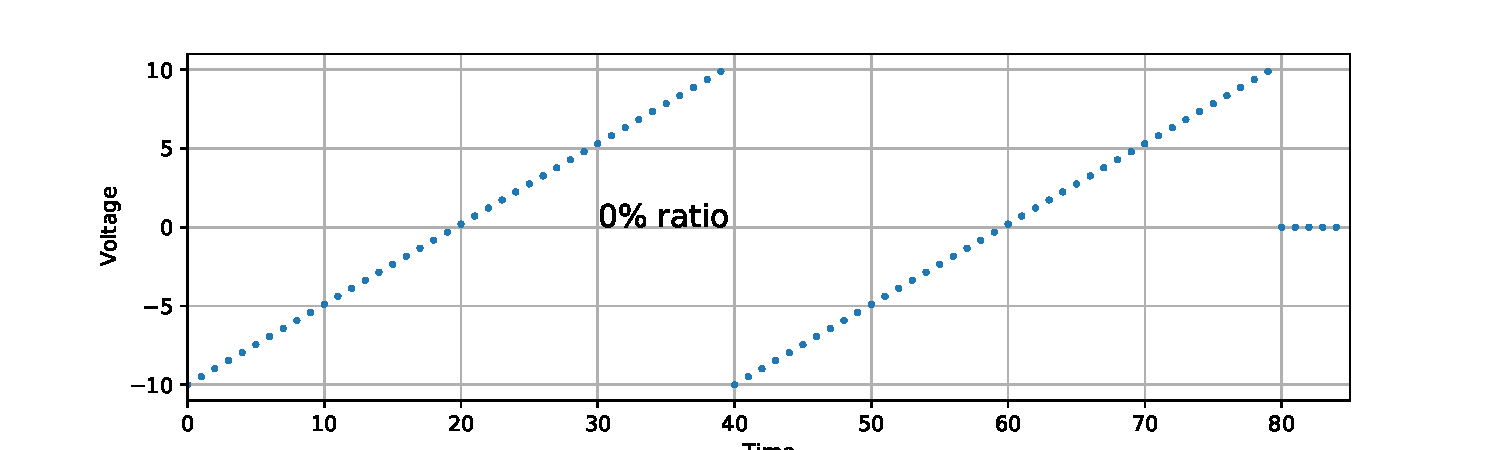
\includegraphics[width=0.95\textwidth]{src/_rampAssymetry0perc.pdf}
		\end{center}
		\begin{center}
		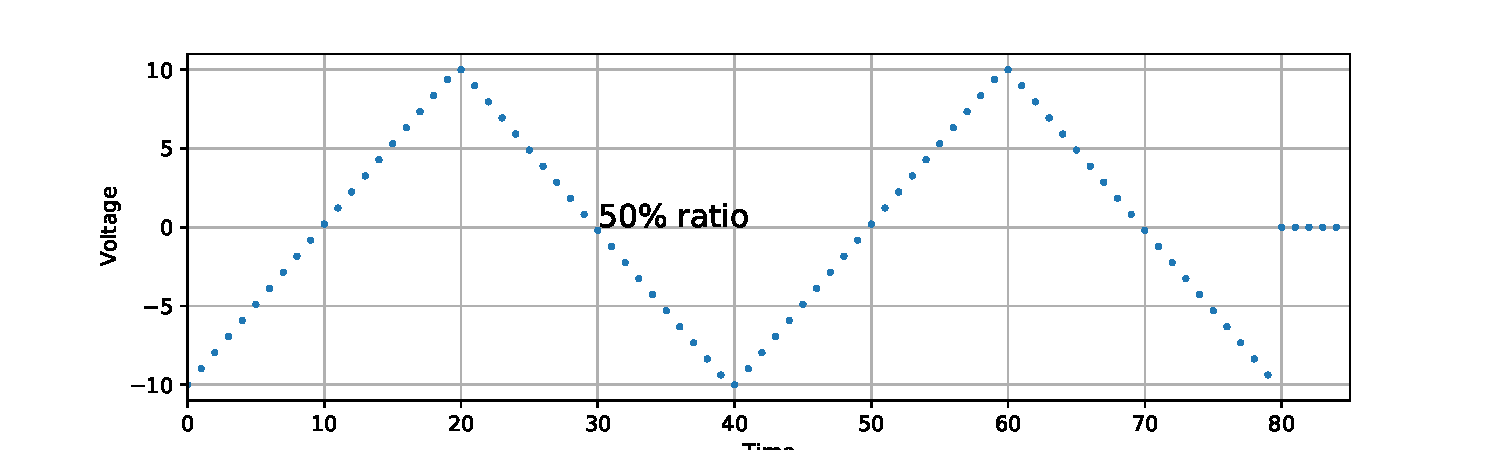
\includegraphics[width=0.95\textwidth]{src/_rampAssymetry50perc.pdf}
		\end{center}
		\begin{center}
		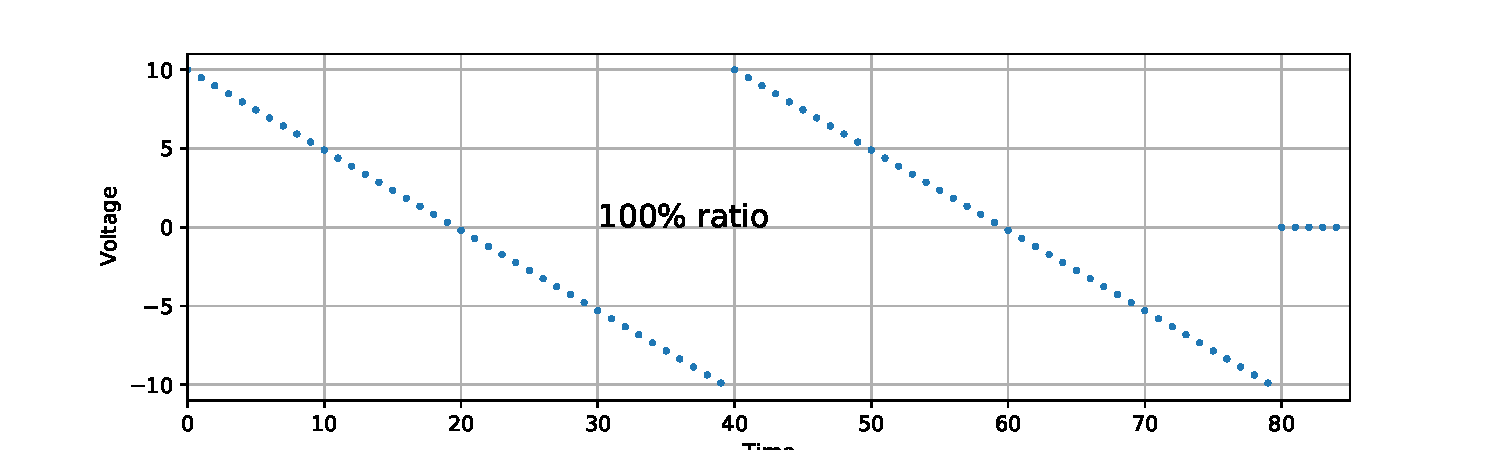
\includegraphics[width=0.95\textwidth]{src/_rampAssymetry100perc.pdf}
		\end{center}


	\req{ RU-21  }{Trigger-IO}{}{}
	{ Internal Trigger-Pulses must be put out via corresponding Trigger-outputs }
	{}{}{}{Triggers}
	\req{ RU-22  }{Trigger-Source}{}{}
	{ Trigger-Modules must be implemented to handle timing of the signal-generation, comprising following input-sources:  $USB$, $Trigger-Input$, $Superior$-$Trigger$, $Push-button$ }
	{}{}{}{Triggers}
	\req{ RU-23  }{Timing-Parameters}{}{}
	{ The FirmWare has to accept signal frequency or signal period and signal vector length as parameters. It has to reply with the actual frequency/period or an error message.}
	{}{}{}{Triggers}
	\req{ RU-24  }{Timing-Calc}{}{}
	{ The FirmWare has to derive necessary sample-rates and trigger-periods from signal period and vector length, either by calculation or by selection from a look-up-table.}
	{}{}{}{Triggers}
	\req{ RU-25  }{Sequences}{}{}
	{ The FirmWare has to generate sequences of A, B and C-Triggers. A-Trigger pulses have a duty-cycle of 50\%, B and C-Trigger have falling edges upon completion.}
	{}{}{}{Triggers}
		\begin{center}
		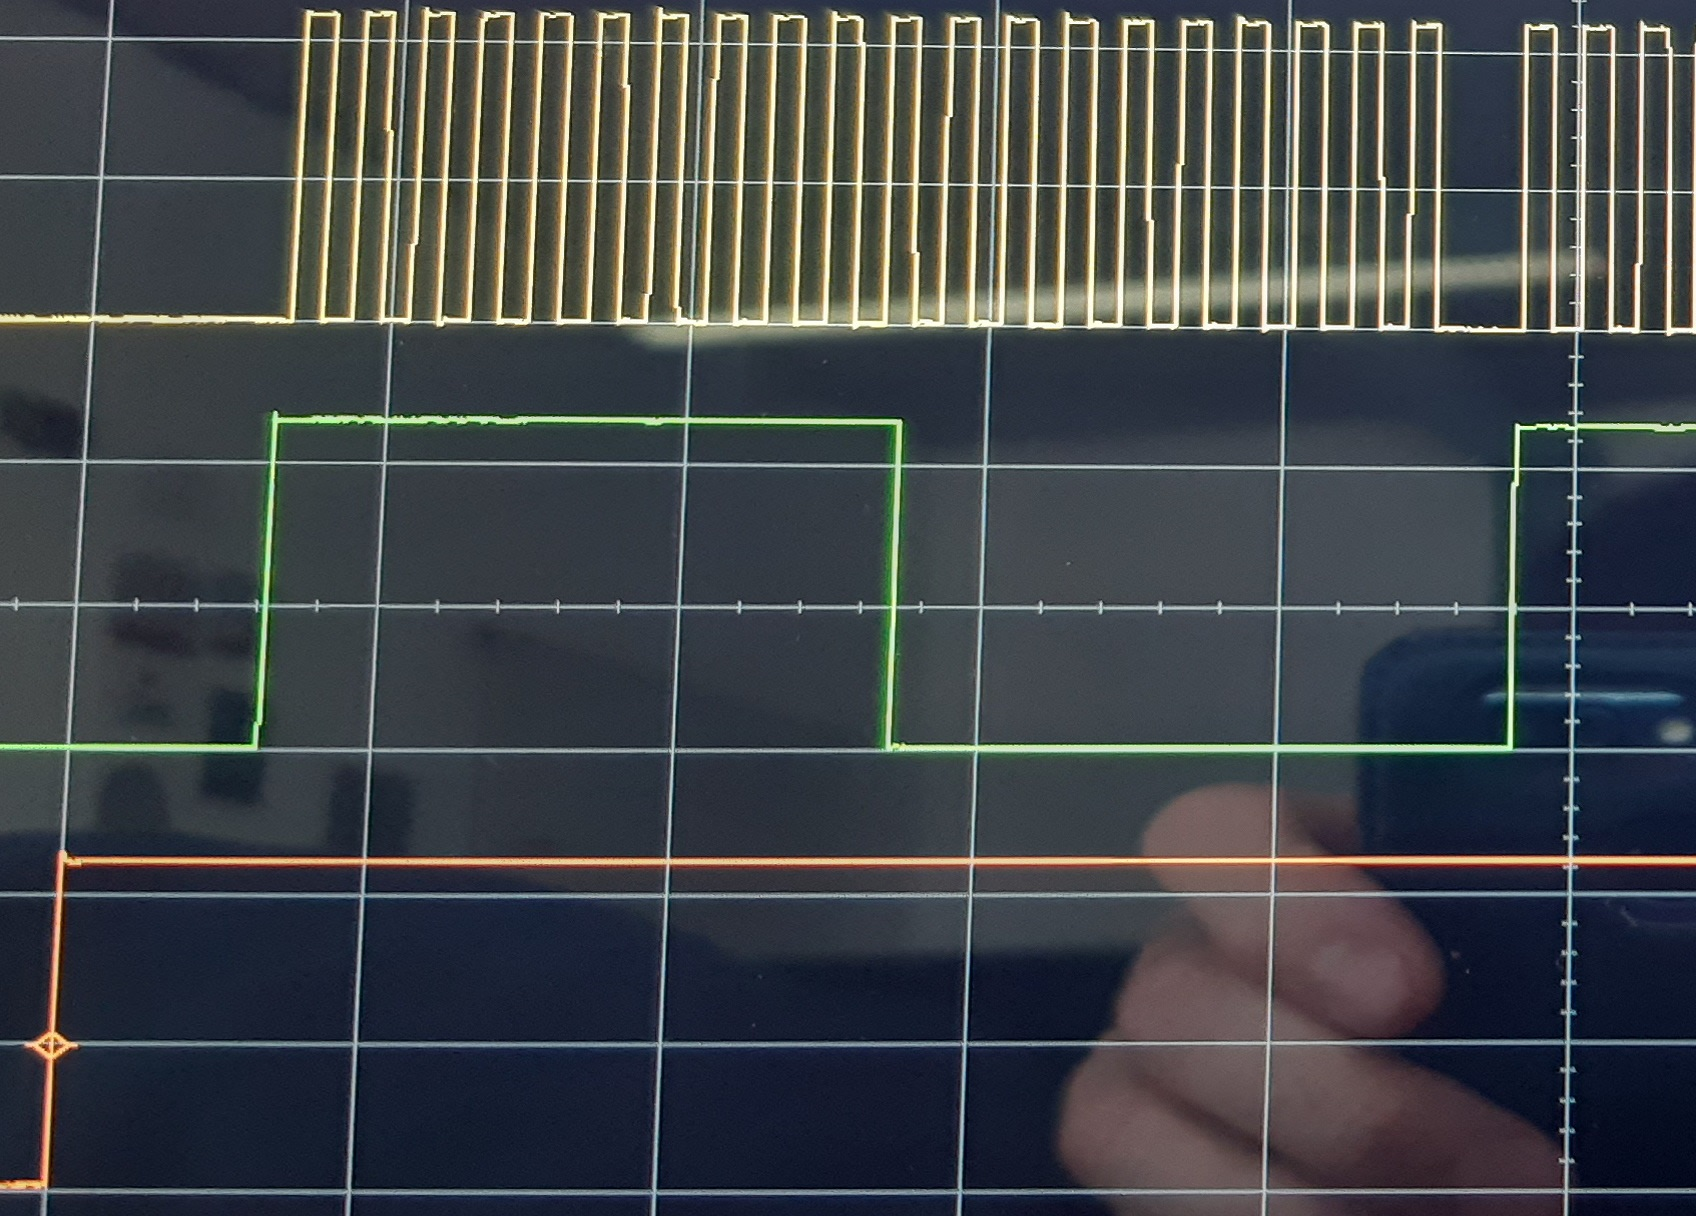
\includegraphics[height=0.2\textheight]{src/_TrigSequence.jpg}
		\end{center}


	\req{ RU-26  }{Buttons,LEDs}{}{}
	{ The FirmWare must access the available push-buttons and state-LEDs. }
	{}{}{}{Miscellaneous}
	\req{ RU-27  }{Button-Function}{}{}
	{ Push-buttons must be programmed to cause transitions to the devices internal state, in a debounced manner. }
	{}{}{}{Miscellaneous}
	\req{ RU-28  }{LED-Function}{}{}
	{ State-LEDs have to represent the current internal state of the device: $idle$, $armed$, $running$ or $error$. }
	{}{}{}{Miscellaneous}
	\req{ RU-29 }{Relays}{}{}
	{ The FirmWare has to provide access to the available relays. Access must consist of $close$, $open$ and $read$-functions }
	{}{}{}{Miscellaneous}
	\req{ RU-30 }{Additional IOs}{}{}
	{ The FirmWare has to provide access for available UART-, $I^2C$-, SPI-modules, as well as digital IOs and analogue inputs.}
	{}{}{}{Miscellaneous}
	\req{ RU-31 }{Additional IO-Modes}{}{}
	{ Functionality for USART-, $I^2C$-, SPI-modules, the digital IOs and analogue inputs must consist of $activation$, $de-activation$, $write$ and $read$.}
	{}{}{}{Miscellaneous}
	\req{ RU-32 }{IO Read}{}{}
	{ $read$-Function must send received information to the host via USB.
	  $read$-Function must be performed upon USB-command, or slave-action.}
	{}{}{}{Miscellaneous}
	\req{ RU-33  }{CRC}{}{}
	{ The FirmWare has to implement functions to perform cyclic-redundancy-check calculations and apply it on verification of incoming strings and adaption of outgoing strings}
	{}{}{}	{Miscellaneous}
	\req{ RU-34  }{Watchdog Functionality \label{WDG}}{ M }{ todo }
	{  The FirmWare has to implement functions to enable the processors built-in watchdog and set its parameters. Available modes have to be $reset$, $powerdown$, $keepalive$}
	{}{}{}	{Miscellaneous}



		\pagebreak
			\subsection{USB-Protocol}
		A direct consequence of the user-requirements is the list of scpi-commands and according replies, forming the USB-protocol.	Scpi-commands can be in 'short form', defined by the capital letters, or in 'long form', defined by the whole string. OCTane accepts both forms as commands and is case-insensitive. \cite{scpi1993}
		{	\scriptsize
					\begin{longtable}{|l|l|l|l|l|}				\hline
		Sub-sys				& Parameter		& Value					& Command									& Response 			\\ \hline
		\redrow	Trigger A	& State			& off|idle|arm|run		& TRIGgerA:STATe	OFF						& <state>|<error>	\\ \hline
							& State			& 						& TRIGgerA:STATe	IDLE					& <state>|<error>	\\ \hline
							& State			& 						& TRIGgerA:STATe	ARM						& <state>|<error>	\\ \hline
							& State			& 						& TRIGgerA:STATe	RUN						& <state>|<error>	\\ \hline
							& Mode (freerun)& finite				& TRIGgerA:MODE		FINite					& <mode> |<error>	\\ \hline
							& Mode 			& infinite				& TRIGgerA:MODE		INFinite				& <mode> |<error>	\\ \hline
							& Input			& USB					& TRIGgerA:INput	USB						& <input>|<error>	\\ \hline
							& Input			& external input		& TRIGgerA:INput	EXTernal				& <input>|<error>	\\ \hline
							& Input			& Trigger B				& TRIGgerA:INput	TRIGgerB				& <input>|<error>	\\ \hline
							& Input			& Trigger C				& TRIGgerA:INput	TRIGgerC				& <input>|<error>	\\ \hline
							& Input			& Button				& TRIGgerA:INput	BUTTon					& <input>|<error>	\\ \hline
							& Signal-Rate	& 1.0e-1 ... 125e3		& TRIGgerA:RATE		<freq>					& <time>|<error>	\\ \hline
							& Signal-Period	& 	8e-6	... 10		& TRIGgerA:PERIod	<time>					& <time>|<error>	\\ \hline
							& Vector-Size	& 1...250000			& TRIGgerA:SIZE		<size>					& <size>|<error>	\\ \hline
		%	Sequencer		& -Gener		& 						& TRIGgerA:									& DONE|		\\ \hline
		\redrow	Trigger B	& State			& off|idle|arm|run		& TRIGgerB:STATe	OFF						& <state>|<error>	\\ \hline
							& State			& 						& TRIGgerB:STATe	IDLE					& <state>|<error>	\\ \hline
							& State			& 						& TRIGgerB:STATe	ARM						& <state>|<error>	\\ \hline
							& State			& 						& TRIGgerB:STATe	RUN						& <state>|<error>	\\ \hline
							& Mode (freerun)& finite				& TRIGgerB:MODE		FINite					& <mode> |<error>	\\ \hline
							& Mode 			& infinite				& TRIGgerB:MODE		INFinite				& <mode> |<error>	\\ \hline
							& Input			& USB					& TRIGgerB:INput	USB						& <input>|<error>	\\ \hline
							& Input			& External				& TRIGgerB:INput	EXTernal				& <input>|<error>	\\ \hline
							& Input			& Trigger C				& TRIGgerB:INput	TRIGgerC				& <input>|<error>	\\ \hline
							& Input			& Button				& TRIGgerB:INput	BUTTon					& <input>|<error>	\\ \hline
							& Signal-Rate	& 	1.0e-1 ... 125e3	& TRIGgerB:RATE		<freq>					& <time>|<error>	\\ \hline
							& Signal-Period	& 	8e-6	... 10		& TRIGgerB:PERIod	<time>					& <time>|<error>	\\ \hline
							& Vector-Size	& 1...250000			& TRIGgerB:SIZE		<size>					& <size>|<error>	\\ \hline
		%	Sequencer		& -Gener		& 						& TRIGgerB:									& DONE|		\\ \hline
		\redrow	Trigger C	& State			& off|idle|arm|run		& TRIGgerC:STATe	OFF						& <state>|<error>	\\ \hline
							& State			& 						& TRIGgerC:STATe	IDLE					& <state>|<error>	\\ \hline
							& State			& 						& TRIGgerC:STATe	ARM						& <state>|<error>	\\ \hline
							& State			& 						& TRIGgerC:STATe	RUN						& <state>|<error>	\\ \hline
							& Mode (freerun)& finite				& TRIGgerC:MODE		FINite					& <mode> |<error>	\\ \hline
							& Mode 			& infinite				& TRIGgerC:MODE		INFinite				& <mode> |<error>	\\ \hline
							& Input			& USB					& TRIGgerC:INput	USB						& <input>|<error>	\\ \hline
							& Input			& External				& TRIGgerC:INput	EXTernal				& <input>|<error>	\\ \hline
							& Input			& Button				& TRIGgerC:INput	BUTTon					& <input>|<error>	\\ \hline
							& Signal-Rate	& 	1.0e-1 ... 125e3	& TRIGgerC:RATE		<freq>					& <time>|<error>	\\ \hline
							& Signal-Period	& 	8e-6	... 10		& TRIGgerC:PERIod	<time>					& <time>|<error>	\\ \hline
							& Vector-Size	& 1...250000			& TRIGgerC:SIZE		<size>					& <size>|<error>	\\ \hline
						% 	& Slope			& rising|falling Edge	& TRIGgerC:SLOPe	<POS|NEG>				& DONE|		\\ \hline
						% 	& Outmode		& pulse|duty			& TRIGgerC:OUTMode	<pulse|duty>			& DONE|		\\ \hline
						% 	& Outpulse		& pulse|duty			& TRIGgerC:OUTPulse	<time>					& DONE|		\\ \hline
						% 	& OutSlope		& rising|falling Edge	& TRIGgerC:OUTSLope	<POS|NEG>				& DONE|		\\ \hline
		%	Sequencer		& -Gener		& 						& TRIGgerC:									& DONE|		\\ \hline
		\redrow	Source-A	& Mode			& triggered				& SOURceA:MODE			TRIGgered			& <mode>|<error> 	\\ \hline
							& Mode			& detached				& SOURceA:MODE			DETached			& <mode>|<error> 	\\ \hline
							& Mode			& singleshot			& SOURceA:MODE			SINGleshot			& <mode>|<error> 	\\ \hline
							& Function		& Ramp					& SOURceA:FUNCtion:SHAPe 	RAMP	 		& <func>|<error>	\\ \hline
							& Function		& 		Arbitrary		& SOURceA:FUNCtion:SHAPe 	ARBitrary 		& <func>|<error>	\\ \hline
							& Symmetry		& 0 ... 100 			& SOURceA:RAMP:RATIO 	<ratio> 			& <ratio>|<error> 	\\ \hline
							& Arb load		& -						& SOURceA:ARBitrary:LOAD 					& <count>|<error>	\\ \hline
							& Arb val		& $\pm$10.000			& SOURceA:ARBitrary:VALUe <idx, val>		& <idx, val>|<error>\\ \hline
							& Amplitude		& 0.000...20.000		& SOURceA:FUNCtion:AMPlitude <ampl>			& <ampl>|<error>	\\ \hline
							& Offset		& $\pm$10.000			& SOURceA:FUNCtion:OFFset <offs>			& <offs>|<error>	\\ \hline
							& High			& $\pm$10.000			& SOURceA:FUNCtion:HIgh <high>				& <high>|<error>	\\ \hline
							& Low			& $\pm$10.000			& SOURceA:FUNCtion:LOw <low>				& <low>|<error> 	\\ \hline
							& Constant		& $\pm$10.000			& SOURceA:VOLTage:LEVel	<volts>				& <volts>|<error> 	\\ \hline
							& Timeout		&  1...1000ms		 	& SOURceA:PULSe:WIDth		<time>			& <time>|<error> 	\\ \hline
						% 	& ReadVec		& -						& SOURceA:ARBitrary:READ					& all vector values \\ \hline
		\redrow	Source-B	& Mode			& trig|det|single		& SOURceB:MODE			TRIGgered			& <mode>|<error> 	\\ \hline
							& Mode			& trig|det|single		& SOURceB:MODE			DETached			& <mode>|<error> 	\\ \hline
							& Mode			& trig|det|single		& SOURceB:MODE			SINGleshot			& <mode>|<error> 	\\ \hline
							& Function		& Ramp					& SOURceB:FUNCtion:SHAPe 	RAMP	 		& <func>|<error>	\\ \hline
							& Function		& Arbitrary				& SOURceB:FUNCtion:SHAPe 	ARBitrary 		& <func>|<error>	\\ \hline
							& Symmetry		& 0 ... 100 			& SOURceB:RAMP:RATIO 	<ratio> 			& <ratio>|<error> 	\\ \hline
							& Arb load		& -						& SOURceB:ARBitrary:LOAD 					& <count>|<error>	\\ \hline
							& Arb val		& $\pm$10.000			& SOURceB:ARBitrary:VALUe <idx, val> 		& <idx, val>|<error>\\ \hline
							& Amplitude		& 0.000...20.000		& SOURceB:FUNCtion:AMPlitude <ampl>			& <ampl>|<error>	\\ \hline
							& Offset		& $\pm$10.000			& SOURceB:FUNCtion:OFFset <offs>			& <offs>|<error>	\\ \hline
							& High			& $\pm$10.000			& SOURceB:FUNCtion:HIgh <high>				& <high>|<error>	\\ \hline
							& Low			& $\pm$10.000			& SOURceB:FUNCtion:LOw <low>				& <low>|<error> 	\\ \hline
							& Constant		& $\pm$10.000			& SOURceB:VOLTage:LEVel	<volts>				& <volts>|<error> 	\\ \hline
							& Timeout		&  1...1000ms		 	& SOURceB:PULSe:WIDth		<time>			& <time>|<error> 	\\ \hline
						% 	& ReadVec		& -						& SOURceB:ARBitrary:READ					& all vector values \\ \hline
		% \redrow	Misc.		& 				& 						& 											&  					\\ \hline
			Relays			& Galvo			& close|open|read		& ROUTe:<CLOSe|OPEN|STATE?> GAL				& <state>|<error>	\\ \hline
							& SLD			& close|open|read		& ROUTe:<CLOSe|OPEN|STATE?> SLD				& <state>|<error>	\\ \hline
							& AIM			& close|open|read		& ROUTe:<CLOSe|OPEN|STATE?> AIM				& <state>|<error>	\\ \hline
							& CAM			& close|open|read		& ROUTe:<CLOSe|OPEN|STATE?> CAM				& <state>|<error>	\\ \hline
						% 	& Sense			& read state			& ROUTe:STATE?	GAL|SLD|AIM|CAM				& <state>|<error>	\\ \hline
						% 	& close			& close Relay			& ROUTe:CLOSe	GAL|SLD|AIM|CAM				& <state>|<error>	\\ \hline
						% 	& open			& open Relay			& ROUTe:OPEN	GAL|SLD|AIM|CAM				& <state>|<error>	\\ \hline
			I2C				& mode			& OFF					& I2C::MODE OFF								& <mode>|<error>	\\ \hline
							& mode			& USB					& I2C::MODE USB								& <mode>|<error>	\\ \hline
							& mode			& slave-action			& I2C::MODE SLAVeaction						& <mode>|<error>	\\ \hline
							& write			& 0 ... 255				& I2C::WRITe <val>							& <val>|<error> 	\\ \hline
							& read			& 0 ... 255				& I2C::READ									& <val>|<error> 	\\ \hline
			UART			& mode			& OFF					& UART:MODE OFF								& <mode>|<error> 	\\ \hline
							& mode			& USB					& UART:MODE USB								& <mode>|<error> 	\\ \hline
							& mode			& slave-IRQ				& UART:MODE SLAVeaction						& <mode>|<error> 	\\ \hline
							& write			& 0 ... 255				& UART:WRITe <val>							& <val>|<error>		\\ \hline
							& read			& 0 ... 255				& UART:READ									& <val>|<error> 	\\ \hline
			DIO				& mode			& OFF			 		& DIGIO:MODE OFF							& <val>|<error>		\\ \hline
							& mode			& input			 		& DIGIO:MODE IN								& <val>|<error>		\\ \hline
							& mode			& output 				& DIGIO:MODE OUT							& <val>|<error>		\\ \hline
							& write			& 0 .. 65535			& DIGIO:WRIte <val>							& <val>|<error>		\\ \hline
							& read			& 0 .. 65535			& DIGIO:READ								& <val>|<error>		\\ \hline
			AnalogIN		& mode			& OFF					& ANAlog0|1|2|3:MODE OFF					& <val>|<error>		\\ \hline
							& mode			& USB					& ANAlog0|1|2|3:MODE USB					& <val>|<error>		\\ \hline
							& mode			& triggered				& ANAlog0|1|2|3:MODE TRIGA					& <val>|<error>		\\ \hline
							& mode			& triggered				& ANAlog0|1|2|3:MODE TRIGB					& <val>|<error>		\\ \hline
							& mode			& triggered				& ANAlog0|1|2|3:MODE TRIGC					& <val>|<error>		\\ \hline
							& read			& 0 ... 4095			& ANAlog0|1|2|3:READ						& <val>|<error>		\\ \hline
		\redrow System		& CRCmode		& OFF					& SYStem:CRC16 OFF							& <state>|<error>	\\ \hline
							& CRCmode		& on					& SYStem:CRC16 ON							& <state>|<error>	\\ \hline
							& ShutDown 		& -						& SYStem:POWerdown							& POWD|<error>	\\ \hline
							& ListSCPI 		& -						& SYStem:LISt								& <list>|<error>	\\ \hline
							& RESEt 		& -						& SYStem:RESEt								& RESE|<error>		\\ \hline
							& RESTart 		& -						& SYStem:RESTart							& REST|<error>	\\ \hline
							& Verbosity		& OFF					& SYStem:VERBose OFF						& <mode>|<error>	\\ \hline
							& Verbosity		& on					& SYStem:VERBose ON							& <mode>|<error>	\\ \hline
							& Watchdog		& OFF					& SYStem:WATchdog OFF						& <mode>|<error>	\\ \hline
							& Watchdog		& on					& SYStem:WATchdog ON						& <mode>|<error>	\\ \hline
							& Time			& 1...1000ms			& SYStem:WATchdog <time>					& <time>|<error>	\\ \hline
			% Encoder		& 	opt. 		& 						& 												& 		& 		\\ \hline
			% Stepper		& 	opt. 		& 						& 												& 		& 		\\ \hline
		\caption{OCTane USB-Protocol, commands}
			\end{longtable}

		% \begin{table}[h!]
			\centering
			\begin{longtable}{|l|l|l|l|l|l|}
			% \begin{tabular}{|p{1.6cm}|l|l|l|l|l|}
			\hline


		Sub-sys					&  Parameter	 	& possible messages	& occurence 						& 			&  \\ \hline
		\redrow	Trigger A|B|C	&  State	 		& TrigX idling|armed|running& sent on every state change 		& 			& 	\\ \hline
				Trigger A|B|C 	& Input				& -200				& error, if button in use			& 			& 	\\ \hline
				Trigger A|B|C 	& Signal-Rate		& -200				& error, if out-of-range			& 			& 	\\ \hline
				Trigger A|B|C 	& Signal-Period		& -200				& error, if out-of-range			& 			& 	\\ \hline
				Trigger A|B|C 	& Vector-Size		& -200				& error, if out-of-range			& 			& 	\\ \hline
		\redrow	Source A|B		& Arb load	 		& -200				& error, if not in Arb-mode			& 			& 	\\ \hline
				Source A|B		& Arb val	 		& VectorX complete	& if sufficient amount of values was sent	& 			& 	\\ \hline
				Source A|B		& Arb val	 		& -200				& error, if out-of-range			& 			& 	\\ \hline
				Source A|B		& Arb val	 		& -200				& error, if exeeds vector-size		& 			& 	\\ \hline
				Source A|B		& Symmetry	 		& -200				& error, if out-of-range			& 			& 	\\ \hline
				Source A|B		& Amplitude			& -200				& error, if out-of-range			& 			& 	\\ \hline
				Source A|B		& Offset			& -200				& error, if out-of-range			& 			& 	\\ \hline
				Source A|B		& High				& -200				& error, if out-of-range			& 			& 	\\ \hline
				Source A|B		& Low				& -200				& error, if out-of-range			& 			& 	\\ \hline
				Source A|B		& Constant			& -200				& error, if out-of-range			& 			& 	\\ \hline
				Source A|B		& Timeout			& -200				& error, if out-of-range			& 			& 	\\ \hline

		\redrow	AIN 			& input value		& AINx: <value>		& sent on every corresp. Trigger	& 			& 	\\ \hline
				DIN 			& input value		& DIN: <value>		& sent on every DIO:READ-Command	& 			& 	\\ \hline
				UART 			& input value		& UART: <value>		& sent on every corresp. Trigger	& 			& 	\\ \hline
				I2C 			& input value		& I2C: <value>		& sent on every corresp. Trigger	& 			& 	\\ \hline
		\caption{OCTane USB-Protocol, responses}
		\label{USB-Protocol-responses}
		\end{longtable}
		% \end{table}

		}
		Table ~\ref{USB-Protocol-responses} specifies the responses by the OCTane, if they are not described sufficiently in the previous table.
		{	\scriptsize
					\begin{longtable}{|l|l|l|l|l|}				\hline
			Command & 	Description									& 	Action	& Return		\\ \hline
			*CLS	& Clear Status Command							& 		& 		\\ \hline
			*ESE & Standard Event Status Enable Command	& 		& 		\\ \hline
			*ESE? & Standard Event Status Enable Query 		& -		& 		\\ \hline
			*ESR? & Standard Event Status Register Query 	& -		& 		\\ \hline
			*IDN? & Identification Query 							& 	-	& ID-String \\ \hline
			*OPC & Operation Complete Command 				& 		& 		\\ \hline
			*OPC? & Operation Complete Query 					& 	-	& 		\\ \hline
			*RST & Reset Command 									& 		& 		\\ \hline
			*SRE & Service Request Enable Command 			& 		& 		\\ \hline
			*SRE? & Service Request Enable Query 				& 	-	& 		\\ \hline
			*STB? & Read Status Byte Query 						& 	-	& Status Byte		\\ \hline
			*TST? & Self-Test Query 									& 	-	& 		\\ \hline
			*WAI & Wait-to-Continue Command 					& 		& 		\\ \hline
			\caption{IEEE 488.2 mandatory commands}
		\end{longtable}
		
		% \begin{longtable}{|l|l|l|l|l|}				\hline
			% Command & 	Description									& 	Action	& Return		\\ \hline
			% *AAD & Accept Address Command						& 		& 		\\ \hline
			% *CAL? & Calibration Query								& 		& 		\\ \hline
			% *DDT & Define Device Trigger Command				& 		& 		\\ \hline
			% *DDT? & Define Device Trigger Query					& 		& 		\\ \hline
			% *DLF & Disable Listener Function Command		& 		& 		\\ \hline
			% *DMC & Define Macro Command						& not imp'd & 		\\ \hline
			% *EMC & Enable Macro Command						& not imp'd & 		\\ \hline
			% *EMC? & Enable Macro Query							& not imp'd & 		\\ \hline
			% *GMC? & Get Macro Contents Query 					& 		& 		\\ \hline
			% *IST? & Individual Status Query						& 		& 		\\ \hline
			% *LMC? & Learn Macro Query								& not imp'd & 		\\ \hline
			% *LRN? & Learn Device Setup Query					& 		& 		\\ \hline
			% *OPT? & Option Identification Query					& 		& 		\\ \hline
			% *PCB & Pass Control Back									& 		& 		\\ \hline
			% *PMC & Purge Macros Command						& not imp'd & 		\\ \hline
			% *PRE & Parallel Poll Enable Register Command	& 		& 		\\ \hline
			% *PRE? & Parallel Poll Enable Register Query		& 		& 		\\ \hline
			% *PSC & Power-On Status Clear Command			& 		& 		\\ \hline
			% *PSC? & Power-On Status Clear Query				& 		& 		\\ \hline
			% *PUD & Protected User Data Command				& 		& 		\\ \hline
			% *PUD? & Protected User Data Query					& 		& 		\\ \hline
			% *RCL & Recall Command									& 		& 		\\ \hline
			% *RDT & Resource Description Transfer Command	& 		& 		\\ \hline
			% *RDT? & Resource Description Transfer Query		& 		& 		\\ \hline
			% *SAV & Save Command									& 		& 		\\ \hline
			% *TRG & Trigger Command									& 		& 		\\ \hline
			% *RMC & Remove Individual Macro Command		& not imp'd & 		\\ \hline
			% *SDS & Save Default Device Settings Command	& 		& 		\\ \hline
			% \caption{IEEE 488.2 optional commands}
		% \end{longtable}
		}
			
		\subsection{Analogue Output Resolution}
		The analogue voltage outputs provide a voltage range of $\pm$10volts, or 20 volts peak-to-peak at a resolution of 16Bit, or $2^{16}$ LSBs \footnote{'least significant bit', the smallest digital value, corresponding with the smallest voltage step}. This requires to decide on a mapping of digital to analogue values. The most obvious mapping would be, to equate -10V with 0 LSB and +10V with 65535 LSB, providing the following resolution:
		\begin{align*}
			\rightarrow 1 LSB \overset{\wedge}{=} U_{LSB} &= \frac{20Vpp}{2^{16}} = 305.17 \mu V \\
		\end{align*}
		Nevertheless, a viable alternative is, to only use 60000 LSB and shift the range towards the centre of the outputs response curve, leading to the following resolution:
		\begin{align*}
			\rightarrow 1 LSB \overset{\wedge}{=} U_{LSB} &= \frac{20Vpp}{60000} = 333.33 \mu V = \frac{1}{3}mV \\
		\end{align*}
		This provides the advantage to cover every exact milli-volt value, which is not possible for the first option, due to quantization. Also, a shift of 3000 LSBs results in considerable headroom in regards to the possible output. This is allows to slightly exceed the required output swing of $\pm$10volts. Therefore, the concluded mapping results to:
		\begin{align*}
			% \textrm{LSB} & \textrm{Voltage} \\
			% 0     &\rightarrow ... \\
			3000LSBs	&\rightarrow -10.000 volts \\
			33000LSBs	&\rightarrow 0.000 volts \\
			63000LSBs	&\rightarrow	10.000 volts \\
			% 65535 &\rightarrow ... \\
		\end{align*}
		% \TODO{Ivan: wie nennt man 1 LSB in digital? HEX-werte?, außerdem wie schreibt man Volt-werte auf English}
		% With the transfer formulas:
		% \begin{align*}
			% \rightarrow 1 LSB \overset{\wedge}{=} U_{LSB} &= \frac{20Vpp}{60000} = 333.33 \mu V = \frac{1}{3}mV \\
			% \rightarrow 1 LSB \overset{\wedge}{=} U_{LSB} &= \frac{20Vpp}{60000} = 333.33 \mu V = \frac{1}{3}mV \\
		% \end{align*}
	% \begin{itemize}
		% \item 0 ... 30000 ... 60000
		% \item 1000 ... 31000 ... 61000
		% \item 2000 ... 32000 ... 62000
		% \item 3000 ... 33000 ... 63000
		% \item 2500 ... 32500 ... 62500
		% \item 0 ... 32767 ... 65535
	% \end{itemize}
	


	\section{Load-Hypothesis, Fault-Hypothesis}
	\section{Traceability-Matrix}
	Linking Requirements by there tags, to the SW-modules, where they are fulfilled
	The traceability Matrix establishes the relations between user requirements and test cases. Furthermore it is good practice to also include requirement IDs inside the source code on the exact point of implementation. The convenient layout for a traceability matrix is to list requirement IDs column-wise, while noting the IDs of the test cases row wise. The reason being that one requirement may have multiple test cases and and it is more convenient to note these multiple IDs in rows, rather than columns.
	\section{V-Model}

	\section{Verification}
	\subsection{Test-cases}
	Automated test-cases are the primary method to ensure code-quality, because they allow for the assessment of functionalities against requirements and produce according documentation of conducted tests. Furthermore, they help identifying  errors in case of failures and secure implemented functionalities during future adaptions. To demonstrate a complete assessment of the firmware, for every existing user-requirement, at least one test-case is necessary. Depending on the depth of examination through the layers of a firmware, test-cases can either be external or internal. \\
	
	External test-cases denote code running on a separate device, controlling and probing the device under test, most useful for a behavioural and user-oriented verification. Internal test-cases are part of the firmware itself, allowing inspection of hardly accessible areas of code. Though running on the target-hardware, these tests also need to transfer test-data onto an external device, capable of storing and report-generation. Best-practice is to apply both approaches according to necessity and even combine them into hybrid test-cases: External code providing input and capturing output, while calling internal test-cases, that can access and deliver information of the device usually inaccessible via production code. \\
	
	Every test-case has to be simple enough, to render verification of the test-code itself unnecessary. First off, to prevent the effort to verify test-code, but also, because explaining test-cases to a customer, who is possibly no programmer, becomes more feasible. A test-case, so complex, that i would require a superordinate test-case, suggests to be split into several cases of lesser respective complexity. \\
			
	In case of commands resulting in digital, analogue or serial output-signals, the according test-case should measure that output and take it into account for the test result. Automated measurement is required if performable with justifiable effort and available measurement instruments. Apart from this method of fully automated testing, few requirements demand assessment in a manual fashion. For example, oscillograms of the resulting analogue signals require evaluation by the eye of a skilled engineer. Automation of this process via spectral analysis or automated comparison with reference signals would require unjustifiable effort, compared to an evaluation via visual inspection. 
	The core purpose of this project is to develop a firmware and not an elaborate test-setup. \\

	Test-cases, usually, belong to one of the following classes: % , \TODO{according to the V-Model}:
	\subsection{Unit-Tests}
		Unit-tests are test-cases that evaluate the correctness of single functions, methods or procedures. A single variable, array or data-set also constitutes such a unit, if the contained data demands deliberate assessment via a test-case. Viable inputs exist in the form of binary values with separate cases for 'true' and 'false'. In case of numerical input, be they of integer or floating-point nature, the boundary-value and equivalence-class methods deliver suitable input values. For inputs in text form, all specified valid texts, and at least one invalid text form a set of useful input values. \cite{jorgensen13}
	\subsection{Integration-Tests}
		The next level of tests concern the interactions between units and their correct cooperation to form correctly working modules and sub-systems. A major focus in integration testing lies on the verification of units and modules to ensure their correct interaction. As this aspect is of a lesser concern during unit-testing, integration-testing is an established branch of verification in its own right. Furthermore, side-effects of units, which are hardly a concern during unit-testing, are important aspects during integration-testing. Testing and demonstrating seamless interoperability and collaboration of modules are the prime objectives. \cite{SpilSoft2005} % \TODO{welche inputs? Oder: beschreibung der integrations-Art nach ISTQB S. 56} Similar to a unit-test for text-driven functions, an integration test has to contain all possible valid inputs and at least one invalid. \\
		The strategy of integration, happening during implementation has significant influence on the design of suitable integration-tests. These are the most common approaches:
		\begin{itemize} \setlength\itemsep{1px}
		\item Top-down integration 
		\item Bottom-up integration 
		\item Ad-hoc integration 
		\item Backbone integration 
	\end{itemize} 


	\subsection{System-Tests}
	% https://de.wikipedia.org/wiki/Heisenbug
	% \TODO{kann ma den da reinschummeln?}	\cite{Beizer95}
	% \subsection{Load/Fault Tests}
	
	% \TODO{cite: IEEE830.pdf, Crowder-REQs, Buttazzo, system-deadlocks (Coffman) und Datenblätter }
	% \subsection{End to end Test}
	% The core concern is if a test is intended and designed as a unit or an end to end test, regardless of additional resources of the system being used.
	% Even though unit tests are not into end-to-end tests they may very well use the outer interfaces of the system under test.

	\subsection{Code Coverage}
	Code Coverage is an accompanying metric to test-cases, indicating their accuracy and completeness of assessment. The goal for this project is to achieve complete statement and branch coverage for the original, self-written source-code. Third-party libraries and HAL-modules from the processor-vendor are excluded from this requirement.
	